% \VignetteIndexEntry{Monocle: Differential expression and time-series analysis for single-cell RNA-Seq and qPCR experiments.} 
% \VignetteEngine{knitr::knitr}
% \VignetteDepends{} 
% \VignettePackage{monocle}
\documentclass[10pt,oneside]{article}\usepackage[]{graphicx}\usepackage[]{color}
%% maxwidth is the original width if it is less than linewidth
%% otherwise use linewidth (to make sure the graphics do not exceed the margin)
\makeatletter
\def\maxwidth{ %
  \ifdim\Gin@nat@width>\linewidth
    \linewidth
  \else
    \Gin@nat@width
  \fi
}
\makeatother

\definecolor{fgcolor}{rgb}{0.345, 0.345, 0.345}
\newcommand{\hlnum}[1]{\textcolor[rgb]{0.686,0.059,0.569}{#1}}%
\newcommand{\hlstr}[1]{\textcolor[rgb]{0.192,0.494,0.8}{#1}}%
\newcommand{\hlcom}[1]{\textcolor[rgb]{0.678,0.584,0.686}{\textit{#1}}}%
\newcommand{\hlopt}[1]{\textcolor[rgb]{0,0,0}{#1}}%
\newcommand{\hlstd}[1]{\textcolor[rgb]{0.345,0.345,0.345}{#1}}%
\newcommand{\hlkwa}[1]{\textcolor[rgb]{0.161,0.373,0.58}{\textbf{#1}}}%
\newcommand{\hlkwb}[1]{\textcolor[rgb]{0.69,0.353,0.396}{#1}}%
\newcommand{\hlkwc}[1]{\textcolor[rgb]{0.333,0.667,0.333}{#1}}%
\newcommand{\hlkwd}[1]{\textcolor[rgb]{0.737,0.353,0.396}{\textbf{#1}}}%

\usepackage{framed}
\makeatletter
\newenvironment{kframe}{%
 \def\at@end@of@kframe{}%
 \ifinner\ifhmode%
  \def\at@end@of@kframe{\end{minipage}}%
  \begin{minipage}{\columnwidth}%
 \fi\fi%
 \def\FrameCommand##1{\hskip\@totalleftmargin \hskip-\fboxsep
 \colorbox{shadecolor}{##1}\hskip-\fboxsep
     % There is no \\@totalrightmargin, so:
     \hskip-\linewidth \hskip-\@totalleftmargin \hskip\columnwidth}%
 \MakeFramed {\advance\hsize-\width
   \@totalleftmargin\z@ \linewidth\hsize
   \@setminipage}}%
 {\par\unskip\endMakeFramed%
 \at@end@of@kframe}
\makeatother

\definecolor{shadecolor}{rgb}{.97, .97, .97}
\definecolor{messagecolor}{rgb}{0, 0, 0}
\definecolor{warningcolor}{rgb}{1, 0, 1}
\definecolor{errorcolor}{rgb}{1, 0, 0}
\newenvironment{knitrout}{}{} % an empty environment to be redefined in TeX

\usepackage{alltt}

\newcommand{\thetitle}{Monocle: Differential expression and time-series analysis for single-cell RNA-Seq and qPCR experiments}

%\usepackage[pdftitle={\thetitle},pdfauthor={Wolfgang Huber}]{whbiocvignette}
\usepackage{whbiocvignette}
% \usepackage{times}
%\usepackage{hyperref}
%\usepackage{verbatim}
%\usepackage{graphicx}
%\usepackage{fancybox}
%\usepackage{color}

\title{\textsf{\textbf{\thetitle}}}
\author{Cole Trapnell\\[1em]University of Washington,\\ Seattle, Washington, USA\\
\texttt{coletrap@uw.edu} \and
Davide Cacchiarelli\\[1em]Harvard University,\\ Cambridge, Massachussetts, USA\\
\texttt{davide@broadinstitute.org}}
\IfFileExists{upquote.sty}{\usepackage{upquote}}{}
\begin{document}



\maketitle

\begin{abstract}
Single cell gene expression studies enable profiling of transcriptional regulation during complex biological processes and within highly hetergeneous cell populations. These studies allow discovery of genes that identify certain subtypes of cells, or that mark a particular intermediate states during a biological process. In many single cell studies, individual cells are executing through a gene expression program in an unsynchronized manner. In effect, each cell is a snapshot of the transcriptional program under study. The package \Rpackage{monocle} provides tools for analyzing single-cell expression experiments. It performs differential gene expression and clustering to identify important genes and cell states. It is designed for RNA-Seq studies, but can be used with qPCR or other targeted assays. For more information on the algorithm at the core of \Rpackage{monocle}, or to learn more about how to use single cell RNA-Seq to study a complex biological process, see Trapnell and Cacchiarelli \emph{et al}\cite{TRAPNELL_CACCHIARELLI}
\end{abstract}

\tableofcontents



\section{Introduction}

The \Rpackage{monocle} package provides a toolkit for analyzing single cell gene expression experiments. It was developed to analyze single cell RNA-seq data, but can also be used with qPCR measurements. This vignette provides an overview of a single cell RNA-Seq analysis workflow with Monocle. Monocle was developed to analyze dynamic biological processes such as cell differentiation, although it also supports simpler experimental settings.

As cells differentiate, they undergo a process of transcriptional re-configuration, with some genes being silenced and others newly activated. While many studies have compared cells at different stages of differentiation, examining intermediate states has proven difficult, for two reasons.  First, it is often not clear from cellular morphology or established markers what intermediate states exist between, for example, a precursor cell type and its terminally differentiated progeny.  Moreover, two cells might transit through a different sequence of intermediate stages and ultimately converge on the same end state.  Second, even cells in a genetically and epigenetically clonal population might progress through differentiation at different rates \emph{in vitro}, depending on positioning and level of contacts with neighboring cells. Looking at average behavior in a group of cells is thus not necessarily faithful to the process through which an individual cell transits.

Monocle computationally reconstructs the transcriptional transitions undergone by differentiating cells.  It orders a mixed, unsynchronized population of cells according to progress through the learned process of differentiation. Because the population may actually differentiate into multiple separate lineages, Monocle allows the process to branch, and can assign each cell to the correct sub-lineage. It subsequently identifies genes which distinguish different states, and genes that are differentially regulated through time. Finally, it performs clustering on all genes, to classify them according to kinetic trends. The algorithm is inspired by and and extends one proposed by Magwene et al to time-order microarray samples \cite{Magwene:2003kq}. Monocle differs from previous work in three ways. First, single-cell RNA-Seq data differ from microarray measurements in many ways, and so Monocle must take special care to model them appropriately at several steps in the algorithm. Secondly, the earlier algorithm assumes that samples progress along a single trajectory through expression space.  However, during cell differentiation, multiple lineages might arise from a single progenitor.  Monocle can find these lineage branches and correctly place cells upon them. Finally, Monocle also performs differential expression analysis and clustering on the ordered cells to help a user identify key events in the biological process of interest.

\section{Single-cell expression data in Monocle}

The \Rpackage{monocle} package takes a matrix of expression values, which are typically for genes (as opposed to splice variants), as calculated by Cufflinks\cite{Trapnell:2012kp} or another gene expression estimation program. Monocle assumes that gene expression values are log-normally distributed, as is typical in RNA-Seq experiments. Monocle does not normalize these expression values to control for library size, depth of sequencing, or other sources of technical variability - whichever program that you use to calculate expression values should do that.  Monocle is \emph{not} meant to be used with raw counts, and doing so could produce nonsense results.   

\subsection{The CellDataSet class}

\Rpackage{monocle} holds single cell expression data in objects of the \Rclass{CellDataSet} class. The class is derived from the Bioconductor \Rclass{ExpressionSet} class, which provides a common interface familiar to those who have analyzed microarray experiments with Bioconductor. The class requires three input files:
\begin{enumerate}
  \item \Robject{exprs}, a numeric matrix of expression values, where rows are genes, and columns are cells
  \item \Robject{phenoData}, an \Rpackage{AnnotatedDataFrame} object, where rows are cells, and columns are cell attributes (such as cell type, culture condition, day captured, etc.)
  \item \Robject{featureData}, an \Rpackage{AnnotatedDataFrame} object, where rows are features (e.g. genes), and columns are gene attributes, such as biotype, gc content, etc.
\end{enumerate}

The expression value matrix \emph{must} have the same number of columns as the \Robject{phenoData} has rows, and it must have the same number of rows as the \Robject{featureData} data frame has rows. Row names of the \Robject{phenoData} object should match the column names of the expression matrix. Row names of the \Robject{featureData} object should match row names of the expression matrix.

You can create a new \Rclass{CellDataSet} object as follows:  

\begin{knitrout}
\definecolor{shadecolor}{rgb}{0.969, 0.969, 0.969}\color{fgcolor}\begin{kframe}
\begin{alltt}
\hlcom{#not run}
\hlstd{HSMM_expr_matrix} \hlkwb{<-} \hlkwd{read.table}\hlstd{(}\hlstr{"fpkm_matrix.txt"}\hlstd{)}
\hlstd{HSMM_sample_sheet} \hlkwb{<-} \hlkwd{read.delim}\hlstd{(}\hlstr{"cell_sample_sheet.txt"}\hlstd{)}
\hlstd{HSMM_gene_annotation} \hlkwb{<-} \hlkwd{read.delim}\hlstd{(}\hlstr{"gene_annotations.txt"}\hlstd{)}
\end{alltt}
\end{kframe}
\end{knitrout}

Once these tables are loaded, you can create the CellDataSet object like this:

\begin{knitrout}
\definecolor{shadecolor}{rgb}{0.969, 0.969, 0.969}\color{fgcolor}\begin{kframe}
\begin{alltt}
\hlstd{pd} \hlkwb{<-} \hlkwd{new}\hlstd{(}\hlstr{"AnnotatedDataFrame"}\hlstd{,} \hlkwc{data} \hlstd{= HSMM_sample_sheet)}
\hlstd{fd} \hlkwb{<-} \hlkwd{new}\hlstd{(}\hlstr{"AnnotatedDataFrame"}\hlstd{,} \hlkwc{data} \hlstd{= HSMM_gene_annotation)}
\hlstd{HSMM} \hlkwb{<-} \hlkwd{newCellDataSet}\hlstd{(}\hlkwd{as.matrix}\hlstd{(HSMM_expr_matrix),} \hlkwc{phenoData} \hlstd{= pd,} \hlkwc{featureData} \hlstd{= fd)}
\end{alltt}
\end{kframe}
\end{knitrout}

This will create a CellDataSet object with expression values measured in FPKM, a measure of relative expression reported by Cufflinks. However, if you performed your single-cell RNA-Seq experiment using \emph{spike-in} standards, you can convert these measurements into mRNAs per cell (RPC), a unit of \emph{absolute} expression. RPC values are often easier to analyze than FPKM values, because have better statistical tools to model them. In some cases, it's possible to convert FPKM values to RPC values even if there were no spike-in standards included in the experiment. You can convert to RPC values before creating your CellDataSet object using the \Robject{relative2abs} function, as follows:

\begin{knitrout}
\definecolor{shadecolor}{rgb}{0.969, 0.969, 0.969}\color{fgcolor}\begin{kframe}
\begin{alltt}
\hlstd{pd} \hlkwb{<-} \hlkwd{new}\hlstd{(}\hlstr{"AnnotatedDataFrame"}\hlstd{,} \hlkwc{data} \hlstd{= HSMM_sample_sheet)}
\hlstd{fd} \hlkwb{<-} \hlkwd{new}\hlstd{(}\hlstr{"AnnotatedDataFrame"}\hlstd{,} \hlkwc{data} \hlstd{= HSMM_gene_annotation)}

\hlcom{# First create a CellDataSet from the relative expression levels}
\hlstd{HSMM} \hlkwb{<-} \hlkwd{newCellDataSet}\hlstd{(HSMM_expr_matrix,}
                       \hlkwc{phenoData} \hlstd{= pd,}
                       \hlkwc{featureData} \hlstd{= fd)}

\hlcom{# Next, use it to estimate RNA counts}
\hlstd{rpc_matrix} \hlkwb{<-} \hlkwd{relative2abs}\hlstd{(HSMM)}

\hlcom{# Now, make a new CellDataSet using the RNA counts}
\hlstd{HSMM} \hlkwb{<-} \hlkwd{newCellDataSet}\hlstd{(rpc_matrix,}
                       \hlkwc{phenoData} \hlstd{= pd,}
                       \hlkwc{featureData} \hlstd{= fd,}
                       \hlkwc{lowerDetectionLimit}\hlstd{=}\hlnum{1}\hlstd{,}
                       \hlkwc{expressionFamily}\hlstd{=}\hlkwd{negbinomial}\hlstd{())}
\end{alltt}
\end{kframe}
\end{knitrout}

Note that since we are using RPC values, we have changed the value of \Robject{lowerDetectionLimit} to reflect the new scale of expression. Importantly, we have also set the \Robject{expressionFamily} to \Robject{negativebin}, which tells Monocle to use the negative binomial distribution in certain downstream statistical tests. Failing to change these two options can create problems later on, so make sure not to forget them when using RPC values.

Finally, we'll also call two functions that pre-calculate some information about the data. Size factors help us normalize for differences in mRNA recovered across cells, and ``dispersion'' values will help us perform differential expression analysis later.
\begin{knitrout}
\definecolor{shadecolor}{rgb}{0.969, 0.969, 0.969}\color{fgcolor}\begin{kframe}
\begin{alltt}
\hlstd{HSMM} \hlkwb{<-} \hlkwd{estimateSizeFactors}\hlstd{(HSMM)}
\hlstd{HSMM} \hlkwb{<-} \hlkwd{estimateDispersions}\hlstd{(HSMM)}
\end{alltt}
\end{kframe}
\end{knitrout}
We're now ready to start using the \Robject{HSMM} object in our analysis.

\section{Quality control of single cell RNA-Seq experiments}
The first step in any single-cell RNA-Seq analysis is identifying poor-quality libraries from further analysis. Most single-cell workflows will include at least some libraries made from dead cells or empty wells in a plate. It's also crucial to remove doublets: libraries that were made from two or more cells accidentally. These cells can disrupt downstream steps like pseudotime ordering or clustering. This section walks through typical quality control steps that should be performed as part of all analyses with Monocle.

It is often convenient to know how many express a particular gene, or how many genes are expressed by a given cell. Monocle provides a simple function to compute those statistics: 
\begin{knitrout}
\definecolor{shadecolor}{rgb}{0.969, 0.969, 0.969}\color{fgcolor}\begin{kframe}
\begin{alltt}
\hlstd{HSMM} \hlkwb{<-} \hlkwd{detectGenes}\hlstd{(HSMM,} \hlkwc{min_expr} \hlstd{=} \hlnum{0.1}\hlstd{)}
\hlkwd{print}\hlstd{(}\hlkwd{head}\hlstd{(}\hlkwd{fData}\hlstd{(HSMM)))}
\end{alltt}
\begin{verbatim}
##                    gene_short_name        biotype num_cells_expressed
## ENSG00000000003.10          TSPAN6 protein_coding                 167
## ENSG00000000005.5             TNMD protein_coding                   0
## ENSG00000000419.8             DPM1 protein_coding                 189
## ENSG00000000457.8            SCYL3 protein_coding                  15
## ENSG00000000460.12        C1orf112 protein_coding                  34
## ENSG00000000938.8              FGR protein_coding                   0
##                    use_for_ordering
## ENSG00000000003.10            FALSE
## ENSG00000000005.5             FALSE
## ENSG00000000419.8             FALSE
## ENSG00000000457.8             FALSE
## ENSG00000000460.12             TRUE
## ENSG00000000938.8             FALSE
\end{verbatim}
\begin{alltt}
\hlstd{expressed_genes} \hlkwb{<-} \hlkwd{row.names}\hlstd{(}\hlkwd{subset}\hlstd{(}\hlkwd{fData}\hlstd{(HSMM), num_cells_expressed} \hlopt{>=} \hlnum{50}\hlstd{))}
\end{alltt}
\end{kframe}
\end{knitrout}

The vector \Robject{expressed\_genes} now holds the identifiers for genes expressed in at least 50 cells of the data set. We will use this list later when we put the cells in order of biological progress. It is also sometimes convenient to exclude genes expressed in few if any cells from the \Rclass{CellDataSet} object so as not to waste CPU time analyzing them for differential expression.

Let's start trying to remove unwanted, poor quality libraries from the CellDataSet. Your single cell RNA-Seq protocol may have given you the opportunity to image individual cells after capture but prior to lysis. This image data allows you to score your cells, confirming that none of your libraries were made from empty wells or wells with excess cell debris.  With some protocols and instruments, you may get more than one cell captured instead just a single cell. You should exclude libraries that you believe did not come from a single cell, if possible. Empty well or debris well libraries can be especially problematic for Monocle. It's also a good idea to check that each cell's RNA-seq library was sequenced to an acceptible degree.  While there is no widely accepted minimum level for what constitutes seequencing ``deeply enough'', use your judgement: a cell sequenced with only a few thousand reads is unlikely to yield meaningful measurements.   

\Rclass{CellDataSet} objects provide a convenient place to store per-cell scoring data: the \Robject{phenoData} slot.  Simply include scoring attributes as columns in the data frome you used to create your \Rclass{CellDataSet} container.  You can then easily filter out cells that don't pass quality control. You might also filter cells based on metrics from high throughput sequencing quality assessment packages such as FastQC. Such tools can often identify RNA-Seq libraries made from heavily degraded RNA, or where the library contains an abnormally large amount of ribosomal, mitochondrial, or other RNA type that you might not be interested in.

The HSMM dataset included with this package has scoring columns built in: 
\begin{knitrout}
\definecolor{shadecolor}{rgb}{0.969, 0.969, 0.969}\color{fgcolor}\begin{kframe}
\begin{alltt}
\hlkwd{print}\hlstd{(}\hlkwd{head}\hlstd{(}\hlkwd{pData}\hlstd{(HSMM)))}
\end{alltt}
\begin{verbatim}
##                Library Well Hours Media Mapped.Fragments Pseudotime State
## T0_CT_A01 SCC10013_A01  A01     0    GM          1958074  23.916673     1
## T0_CT_A03 SCC10013_A03  A03     0    GM          1930722   9.022265     1
## T0_CT_A05 SCC10013_A05  A05     0    GM          1452623   7.546608     1
## T0_CT_A06 SCC10013_A06  A06     0    GM          2566325  21.463948     1
## T0_CT_A07 SCC10013_A07  A07     0    GM          2383438  11.299806     1
## T0_CT_A08 SCC10013_A08  A08     0    GM          1472238  67.436042     2
##           Size_Factor num_genes_expressed
## T0_CT_A01   2.8512907                9957
## T0_CT_A03   1.3362363                7250
## T0_CT_A05   1.0439424                6049
## T0_CT_A06   0.8975817                5065
## T0_CT_A07   0.8570724                4494
## T0_CT_A08   1.0212473                5359
\end{verbatim}
\end{kframe}
\end{knitrout}

This dataset has already been filtered using the following commands: 

\begin{knitrout}
\definecolor{shadecolor}{rgb}{0.969, 0.969, 0.969}\color{fgcolor}\begin{kframe}
\begin{alltt}
\hlstd{valid_cells} \hlkwb{<-} \hlkwd{row.names}\hlstd{(}\hlkwd{subset}\hlstd{(}\hlkwd{pData}\hlstd{(HSMM), Cells.in.Well} \hlopt{==} \hlnum{1} \hlopt{&} \hlstd{Control} \hlopt{==} \hlnum{FALSE} \hlopt{&} \hlstd{Clump} \hlopt{==} \hlnum{FALSE} \hlopt{&} \hlstd{Debris} \hlopt{==} \hlnum{FALSE} \hlopt{&} \hlstd{Mapped.Fragments} \hlopt{>} \hlnum{1000000}\hlstd{))}
\hlstd{HSMM} \hlkwb{<-} \hlstd{HSMM[,valid_cells]}
\end{alltt}
\end{kframe}
\end{knitrout}

If you are using RPC values to measure expresion, as we are in this vignette, it's also good to look at the distribution of mRNA totals across the cells:
\begin{knitrout}
\definecolor{shadecolor}{rgb}{0.969, 0.969, 0.969}\color{fgcolor}\begin{kframe}
\begin{alltt}
\hlkwd{pData}\hlstd{(HSMM)}\hlopt{$}\hlstd{Total_mRNAs} \hlkwb{<-} \hlkwd{colSums}\hlstd{(}\hlkwd{exprs}\hlstd{(HSMM))}

\hlkwd{qplot}\hlstd{(Total_mRNAs,} \hlkwc{data}\hlstd{=}\hlkwd{pData}\hlstd{(HSMM),} \hlkwc{color}\hlstd{=Hours,} \hlkwc{geom}\hlstd{=}\hlstr{"density"}\hlstd{)} \hlopt{+}
  \hlkwd{geom_vline}\hlstd{(}\hlkwc{xintercept}\hlstd{=}\hlnum{10000}\hlstd{)} \hlopt{+}
  \hlkwd{geom_vline}\hlstd{(}\hlkwc{xintercept}\hlstd{=}\hlnum{40000}\hlstd{)}
\end{alltt}
\end{kframe}

{\centering 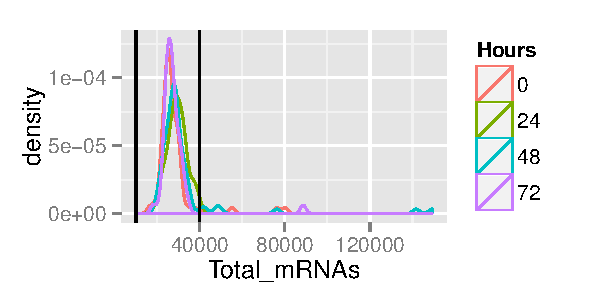
\includegraphics[width=\maxwidth]{figure/show_mRNA_totals-1} 

}


\begin{kframe}\begin{alltt}
\hlstd{HSMM} \hlkwb{<-} \hlstd{HSMM[,}\hlkwd{row.names}\hlstd{(}\hlkwd{subset}\hlstd{(}\hlkwd{pData}\hlstd{(HSMM), Total_mRNAs} \hlopt{>=} \hlnum{10000} \hlopt{&} \hlstd{Total_mRNAs} \hlopt{<=} \hlnum{40000}\hlstd{))]}
\hlstd{HSMM} \hlkwb{<-} \hlkwd{detectGenes}\hlstd{(HSMM,} \hlkwc{min_expr} \hlstd{=} \hlnum{0.1}\hlstd{)}
\end{alltt}
\end{kframe}
\end{knitrout}

We've gone ahead and removed the few cells with either very low mRNA recovery or far more mRNA that the typical cell. Often, doublets or triplets have roughly twice the mRNA recovered as true single cells, so the latter filter is another means of excluding all but single cells from the analysis. Such filtering is handy if your protocol doesn't allow directly visualization of cell after they've been captured.

Once you've excluded cells that do not pass your quality control filters, you should verify that the expression values stored in your \Rclass{CellDataSet} follow a distribution that is roughly lognormal:  
\begin{knitrout}
\definecolor{shadecolor}{rgb}{0.969, 0.969, 0.969}\color{fgcolor}\begin{kframe}
\begin{alltt}
\hlcom{# Log-transform each value in the expression matrix.}
\hlstd{L} \hlkwb{<-} \hlkwd{log}\hlstd{(}\hlkwd{exprs}\hlstd{(HSMM[expressed_genes,]))}

\hlcom{# Standardize each gene, so that they are all on the same scale,}
\hlcom{# Then melt the data with plyr so we can plot it easily"}
\hlstd{melted_dens_df} \hlkwb{<-} \hlkwd{melt}\hlstd{(}\hlkwd{t}\hlstd{(}\hlkwd{scale}\hlstd{(}\hlkwd{t}\hlstd{(L))))}

\hlcom{# Plot the distribution of the standardized gene expression values.}
\hlkwd{qplot}\hlstd{(value,} \hlkwc{geom}\hlstd{=}\hlstr{"density"}\hlstd{,} \hlkwc{data}\hlstd{=melted_dens_df)} \hlopt{+}  \hlkwd{stat_function}\hlstd{(}\hlkwc{fun} \hlstd{= dnorm,} \hlkwc{size}\hlstd{=}\hlnum{0.5}\hlstd{,} \hlkwc{color}\hlstd{=}\hlstr{'red'}\hlstd{)} \hlopt{+}
\hlkwd{xlab}\hlstd{(}\hlstr{"Standardized log(FPKM)"}\hlstd{)} \hlopt{+}
\hlkwd{ylab}\hlstd{(}\hlstr{"Density"}\hlstd{)}
\end{alltt}


{\ttfamily\noindent\color{warningcolor}{\#\# Warning: Removed 1804710 rows containing non-finite values (stat\_density).}}\end{kframe}

{\centering 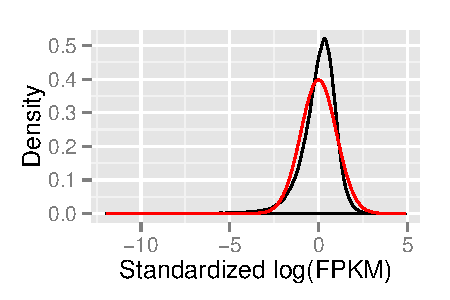
\includegraphics[width=\maxwidth]{figure/lognormal_plot-1} 

}



\end{knitrout}

\section{Identifying cells of interest}

Single cell experiments are often performed on complex mixtures of multiple cell types. Dissociated tissue samples might contain two, three, or even many different cells types. In such cases, it's often nice to classify cells based on type using known markers. In the myoblast experiment, the culture contains fibroblasts that came from the original muscle biopsy used to establish the primary cell culture.  Myoblasts express some key genes that fibroblasts don't. Selecting only the genes that express, for example, sufficiently high levels of \emph{MYF5} or \emph{MEF2C} excludes the fibroblasts. In the block of code below we first grab the values of \emph{MYF5} and \emph{MEF2C} for each cell, and then set these as columns in the pData table for the HSMM object.  We don't have to do this, but it makes filtering a little more convenient. Next we create a vector that has a boolean flag for each cell: TRUE for a myoblast, false for a fibroblast. We then use that vector to creat a third column in the that specicies each cell's type. Finally, we subset the CellDataSet object to create $HSMM_myo$, which includes only myoblasts.  

\begin{knitrout}
\definecolor{shadecolor}{rgb}{0.969, 0.969, 0.969}\color{fgcolor}\begin{kframe}
\begin{alltt}
\hlstd{MEF2C_expr} \hlkwb{<-} \hlkwd{exprs}\hlstd{(HSMM[}\hlkwd{row.names}\hlstd{(}\hlkwd{subset}\hlstd{(}\hlkwd{fData}\hlstd{(HSMM), gene_short_name} \hlopt{==} \hlstr{"MEF2C"}\hlstd{)),])}
\hlstd{MYF5_expr} \hlkwb{<-} \hlkwd{exprs}\hlstd{(HSMM[}\hlkwd{row.names}\hlstd{(}\hlkwd{subset}\hlstd{(}\hlkwd{fData}\hlstd{(HSMM), gene_short_name} \hlopt{==} \hlstr{"MYF5"}\hlstd{)),])}

\hlkwd{pData}\hlstd{(HSMM)}\hlopt{$}\hlstd{MEF2C} \hlkwb{<-} \hlkwd{as.vector}\hlstd{(MEF2C_expr)}
\hlkwd{pData}\hlstd{(HSMM)}\hlopt{$}\hlstd{MYF5} \hlkwb{<-} \hlkwd{as.vector}\hlstd{(MYF5_expr)}

\hlstd{MEF2C_thresh} \hlkwb{<-} \hlnum{5} \hlcom{#0.1}
\hlstd{MYF5_thresh} \hlkwb{<-} \hlnum{1} \hlcom{#0.1}

\hlcom{#cell_is_hsmm <- (pData(HSMM)$MEF2C > MEF2C_thresh | pData(HSMM)$MYF5 > MYF5_thresh) }
\hlstd{cell_is_hsmm} \hlkwb{<-} \hlstd{(}\hlkwd{pData}\hlstd{(HSMM)}\hlopt{$}\hlstd{MEF2C} \hlopt{>} \hlstd{MEF2C_thresh} \hlopt{|} \hlkwd{pData}\hlstd{(HSMM)}\hlopt{$}\hlstd{MYF5} \hlopt{>} \hlstd{MYF5_thresh)}

\hlkwd{names}\hlstd{(cell_is_hsmm)} \hlkwb{<-} \hlkwd{row.names}\hlstd{(}\hlkwd{pData}\hlstd{(HSMM))}
\hlkwd{pData}\hlstd{(HSMM)}\hlopt{$}\hlstd{CellType} \hlkwb{<-} \hlstr{"Myoblast"}
\hlkwd{pData}\hlstd{(HSMM)}\hlopt{$}\hlstd{CellType[cell_is_hsmm} \hlopt{==} \hlnum{FALSE}\hlstd{]} \hlkwb{<-}  \hlstr{"Fibroblast"}

\hlstd{HSMM_myo} \hlkwb{<-} \hlstd{HSMM[,}\hlkwd{pData}\hlstd{(HSMM)}\hlopt{$}\hlstd{CellType} \hlopt{==} \hlstr{"Myoblast"}\hlstd{]}
\end{alltt}
\end{kframe}
\end{knitrout}

Now that we have tagged the cells, it's easy to quantify the level of fibroblast ``contaminantation'' in the HSMM culture:

\begin{knitrout}
\definecolor{shadecolor}{rgb}{0.969, 0.969, 0.969}\color{fgcolor}\begin{kframe}
\begin{alltt}
\hlstd{pie} \hlkwb{<-} \hlkwd{ggplot}\hlstd{(}\hlkwd{pData}\hlstd{(HSMM),} \hlkwd{aes}\hlstd{(}\hlkwc{x} \hlstd{=} \hlkwd{factor}\hlstd{(}\hlnum{1}\hlstd{),} \hlkwc{fill} \hlstd{=} \hlkwd{factor}\hlstd{(CellType)))} \hlopt{+}
 \hlkwd{geom_bar}\hlstd{(}\hlkwc{width} \hlstd{=} \hlnum{1}\hlstd{)}
\hlstd{pie} \hlopt{+} \hlkwd{coord_polar}\hlstd{(}\hlkwc{theta} \hlstd{=} \hlstr{"y"}\hlstd{)} \hlopt{+}
  \hlkwd{theme}\hlstd{(}\hlkwc{axis.title.x}\hlstd{=}\hlkwd{element_blank}\hlstd{(),} \hlkwc{axis.title.y}\hlstd{=}\hlkwd{element_blank}\hlstd{())}
\end{alltt}
\end{kframe}

{\centering 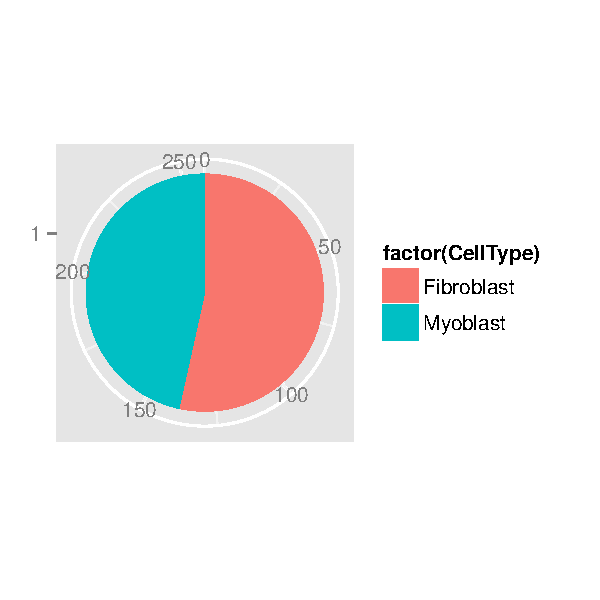
\includegraphics[width=\maxwidth]{figure/cell_type_pie-1} 

}



\end{knitrout}

\section{Basic differential expression analysis}

Differential gene expression analysis is a common task in RNA-Seq experiments.  Monocle can help you find genes that are differentially expressed between groups of cells and assesses the statistical signficance of those changes. These comparisons require that you have a way to collect your cells into two or more groups.  These groups are defined by columns in the \Robject{phenoData} table of each \Robject{CellDataSet}.  Monocle will assess the signficance of each gene's expression level across the different groups of cells.

Performing differential expression analysis on all genes in the human genome can take a substantial amount of time. For a dataset as large as the myoblast data from \cite{TRAPNELL_CACCHIARELLI}, which contains several hundred cells, the analysis can take several hours on a single CPU. Let's select a small set of genes that we know are important in myogenesis to demonstrate Monocle's capabilities: 
\begin{knitrout}
\definecolor{shadecolor}{rgb}{0.969, 0.969, 0.969}\color{fgcolor}\begin{kframe}
\begin{alltt}
\hlstd{marker_genes} \hlkwb{<-} \hlkwd{row.names}\hlstd{(}\hlkwd{subset}\hlstd{(}\hlkwd{fData}\hlstd{(HSMM_myo),}
                                 \hlstd{gene_short_name} \hlopt \hlkwd{c}\hlstd{(}\hlstr{"MEF2C"}\hlstd{,} \hlstr{"MEF2D"}\hlstd{,} \hlstr{"MYF5"}\hlstd{,}
                                                        \hlstr{"ANPEP"}\hlstd{,} \hlstr{"PDGFRA"}\hlstd{,}\hlstr{"MYOG"}\hlstd{,}
                                                        \hlstr{"TPM1"}\hlstd{,}  \hlstr{"TPM2"}\hlstd{,}  \hlstr{"MYH2"}\hlstd{,}
                                                        \hlstr{"MYH3"}\hlstd{,}  \hlstr{"NCAM1"}\hlstd{,} \hlstr{"TNNT1"}\hlstd{,}
                                                        \hlstr{"TNNT2"}\hlstd{,} \hlstr{"TNNC1"}\hlstd{,} \hlstr{"CDK1"}\hlstd{,}
                                                        \hlstr{"CDK2"}\hlstd{,}  \hlstr{"CCNB1"}\hlstd{,} \hlstr{"CCNB2"}\hlstd{,}
                                                        \hlstr{"CCND1"}\hlstd{,} \hlstr{"CCNA1"}\hlstd{,} \hlstr{"ID1"}\hlstd{)))}
\end{alltt}
\end{kframe}
\end{knitrout}

In the myoblast data, the cells collected at the outset of the experiment were cultured in ``growth medium'' (GM) to prevent them from differentiating.  After they were harvested, the rest of the cells were switched over to ``differentiation medium'' (DM) to promote differentiation. Let's have monocle find which of the genes above are affected by this switch:
\begin{knitrout}
\definecolor{shadecolor}{rgb}{0.969, 0.969, 0.969}\color{fgcolor}\begin{kframe}
\begin{alltt}
\hlstd{diff_test_res} \hlkwb{<-} \hlkwd{differentialGeneTest}\hlstd{(HSMM_myo[marker_genes,],}
                                      \hlkwc{fullModelFormulaStr}\hlstd{=}\hlstr{"~Media"}\hlstd{)}

\hlcom{# Select genes that are significant at an FDR < 10%}
\hlstd{sig_genes} \hlkwb{<-} \hlkwd{subset}\hlstd{(diff_test_res, qval} \hlopt{<} \hlnum{0.1}\hlstd{)}

\hlstd{sig_genes[,}\hlkwd{c}\hlstd{(}\hlstr{"gene_short_name"}\hlstd{,} \hlstr{"pval"}\hlstd{,} \hlstr{"qval"}\hlstd{)]}
\end{alltt}
\begin{verbatim}
##                    gene_short_name         pval         qval
## ENSG00000081189.9            MEF2C 1.488239e-08 7.813256e-08
## ENSG00000105048.12           TNNT1 5.191657e-05 1.211387e-04
## ENSG00000109063.9             MYH3 8.213617e-06 2.156075e-05
## ENSG00000111049.3             MYF5 7.182938e-10 5.028057e-09
## ENSG00000114854.3            TNNC1 2.762425e-06 9.668487e-06
## ENSG00000118194.14           TNNT2 1.269131e-16 2.665175e-15
## ENSG00000122180.4             MYOG 4.191264e-03 6.286896e-03
## ENSG00000123374.6             CDK2 3.233138e-03 5.222761e-03
## ENSG00000125414.13            MYH2 1.193437e-03 2.088514e-03
## ENSG00000125968.7              ID1 7.132934e-08 2.995832e-07
## ENSG00000134057.10           CCNB1 2.810908e-02 3.689316e-02
## ENSG00000140416.15            TPM1 3.923939e-06 1.177182e-05
## ENSG00000149294.12           NCAM1 1.157988e-15 1.215888e-14
## ENSG00000157456.3            CCNB2 8.315063e-04 1.587421e-03
## ENSG00000166825.9            ANPEP 6.102415e-03 8.543381e-03
## ENSG00000198467.8             TPM2 5.289995e-04 1.110899e-03
\end{verbatim}
\end{kframe}
\end{knitrout}

So 16 of the 22 genes are significant at a 10\% false discovery rate! This isn't surprising, as most of the above genes are highly relevant in myogenesis. Monocle also provides some easy ways to plot the expression of a small set of genes grouped by the factors you use during differential analysis.  This helps you visualize the differences revealed by the tests above.  One type of plot is a ``jitter'' plot.

\begin{knitrout}
\definecolor{shadecolor}{rgb}{0.969, 0.969, 0.969}\color{fgcolor}\begin{kframe}
\begin{alltt}
\hlstd{MYOG_ID1} \hlkwb{<-} \hlstd{HSMM_myo[}\hlkwd{row.names}\hlstd{(}\hlkwd{subset}\hlstd{(}\hlkwd{fData}\hlstd{(HSMM_myo),}
                                 \hlstd{gene_short_name} \hlopt \hlkwd{c}\hlstd{(}\hlstr{"MYOG"}\hlstd{,} \hlstr{"CCNB2"}\hlstd{))),]}
\hlkwd{plot_genes_jitter}\hlstd{(MYOG_ID1,} \hlkwc{grouping}\hlstd{=}\hlstr{"Media"}\hlstd{,} \hlkwc{ncol}\hlstd{=}\hlnum{2}\hlstd{)}
\end{alltt}
\end{kframe}

{\centering 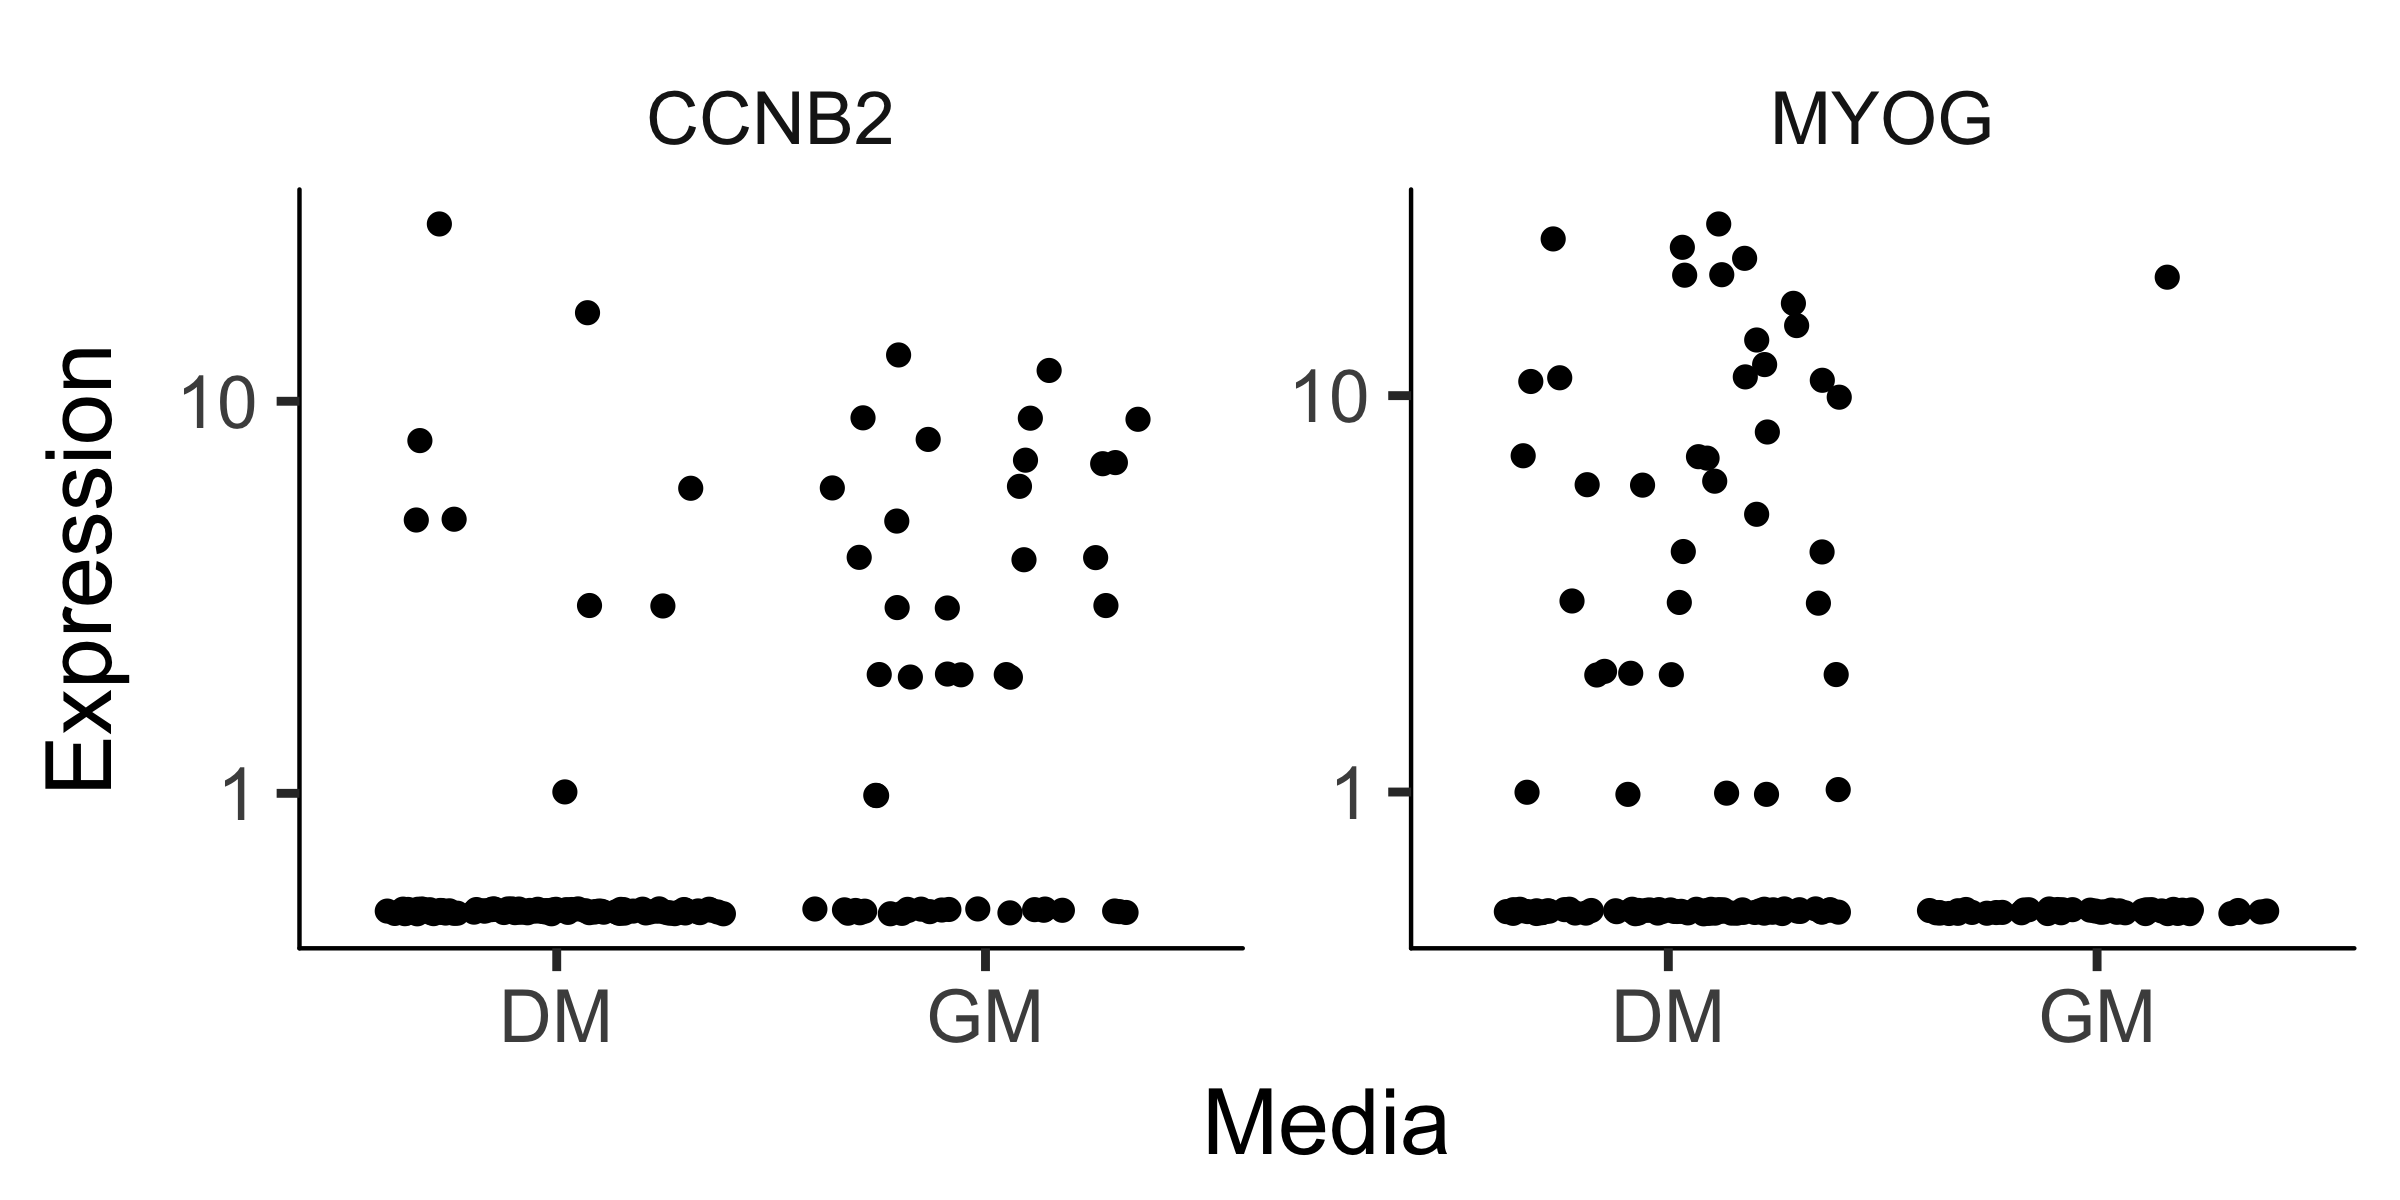
\includegraphics[width=\maxwidth]{figure/plot_myog_jitter-1} 

}



\end{knitrout}

Note that we can control how to layout the genes in the plot by specifying the number of rows and columns.  See the man page on \Rfunction{plot\_genes\_jitter} for more details on controlling its layout. Most if not all of Monocle's plotting routines return a plot object from the \Rpackage{ggplot2}.  This package uses a grammar of graphics to control various aspects of a plot, and makes it easy to customize how your data is presented.  See the \Rpackage{ggplot2} book\cite{Wickham} for more details.

\section{Ordering cells by progress in ``pseudotime''}

In many biological processes, cells do not progress in perfect synchrony.  In single-cell expression studies of processes such as cell differentiation, captured cells might be widely distributed in terms of progress.  That is, in a population of cells captured at exactly the same time, some cells might be far along, while others might not yet even have begun the process.  Monocle can informatically put the cells ``in order'' of how far they have progressed through the process you're studying.  Monocle may even be able to find where cells diverge, with groups of cells proceeding down distinct paths.  In this section, we will put a set of differentiating myoblasts in order of progress through myogenesis. 

First, we must decide which genes we will use to define a cell's progress through myogenesis. Monocle orders cells by examining the pattern of expression of these genes across the cell population.  Monocle looks for genes that vary in ``interesting'' ways (that is aren't just noisy), and uses these to structure the data. We ultimately want a set of genes that increase (or decrease) in expression as a function of progress through the process we're studying. 

Ideally, we'd like to use as little prior knowledge of the biology of the system under study as possible. We'd like to discover the important ordering genes from the data, rather than relying on literature and textbooks, because that might introduce bias in the ordering. One effective way to isolate a set of ordering genes is to simply compare the cells collected at the beginning of the process to those at the end and find the differentially expressed genes, as described above. The command below will find all genes that are differentially expressed in response to the switch from growth medium to differentiation medium:

\begin{knitrout}
\definecolor{shadecolor}{rgb}{0.969, 0.969, 0.969}\color{fgcolor}\begin{kframe}
\begin{alltt}
\hlcom{#not run}
\hlstd{diff_test_res} \hlkwb{<-} \hlkwd{differentialGeneTest}\hlstd{(HSMM_myo[expressed_genes,],} \hlkwc{fullModelFormulaStr}\hlstd{=}\hlstr{"~Media"}\hlstd{)}
\hlstd{ordering_genes} \hlkwb{<-} \hlkwd{row.names} \hlstd{(}\hlkwd{subset}\hlstd{(diff_test_res, qval} \hlopt{<} \hlnum{0.01}\hlstd{))}
\end{alltt}
\end{kframe}
\end{knitrout}

We could also leverage the developmental biology community's extensive knowledge of expression dynamics during skeletal myogenesis, and use the small set of genes discussed above. 

\begin{knitrout}
\definecolor{shadecolor}{rgb}{0.969, 0.969, 0.969}\color{fgcolor}\begin{kframe}
\begin{alltt}
\hlcom{#not run}
\hlstd{ordering_genes} \hlkwb{<-} \hlkwd{intersect} \hlstd{(marker_genes, expressed_genes)}
\end{alltt}
\end{kframe}
\end{knitrout}

In most cases, however, we want to use all genes that are expressed above a reasonable threshold. Including genes that are expressed at extremely low levels in only a few cells just injects noise into the ordering analysis, so we'll exclude them. Monocle provides a function to collect the list of genes that are expressed above or below given thresholds. The function \Robject{selectGenesInExpressionRange} allows you to select genes that have, for example, a median expression level across cells of at least 2 RPC. This function is quite flexible: see the man page for ?selectGenesInExpressionRange for more details

\begin{knitrout}
\definecolor{shadecolor}{rgb}{0.969, 0.969, 0.969}\color{fgcolor}\begin{kframe}
\begin{alltt}
\hlstd{ordering_genes} \hlkwb{<-} \hlkwd{selectGenesInExpressionRange}\hlstd{(HSMM_myo,}
                                               \hlkwc{min_expression_threshold}\hlstd{=}\hlnum{2}\hlstd{,}
                                               \hlkwc{max_expression_threshold}\hlstd{=}\hlnum{Inf}\hlstd{,}
                                               \hlkwc{detectionLimit}\hlstd{=}\hlnum{0.1}\hlstd{,}
                                               \hlkwc{stat_fun}\hlstd{=}\hlkwa{function}\hlstd{(}\hlkwc{x}\hlstd{) \{} \hlkwd{median}\hlstd{(}\hlkwd{round}\hlstd{(x)) \})}
\end{alltt}
\end{kframe}
\end{knitrout}

Once we have a list of gene ids to be used for ordering, we need to set them in the \Robject{HSMM} object, because the next several functions will depend on them.

\begin{knitrout}
\definecolor{shadecolor}{rgb}{0.969, 0.969, 0.969}\color{fgcolor}\begin{kframe}
\begin{alltt}
\hlstd{HSMM_myo} \hlkwb{<-} \hlkwd{setOrderingFilter}\hlstd{(HSMM_myo, ordering_genes)}
\end{alltt}
\end{kframe}
\end{knitrout}

The genes we've chosen to use for ordering define the \emph{state space} of the cells in our data set.  Each cell is a point in this space, which has dimensionality equal to the number of genes we've chosen.  So if there are 500 genes used for ordering, each cell is a point in a 500-dimensional space.  For a number of reasons, Monocle works better if we can \emph{reduce} the dimensionality of that space before we try to put the cells in order.  In this case, we will reduce the space down to one with two dimensions, which we will be able to easily visualize and interpret while Monocle is ordering the cells.
\begin{knitrout}
\definecolor{shadecolor}{rgb}{0.969, 0.969, 0.969}\color{fgcolor}\begin{kframe}
\begin{alltt}
\hlstd{HSMM_myo} \hlkwb{<-} \hlkwd{reduceDimension}\hlstd{(HSMM_myo)}
\end{alltt}
\end{kframe}
\end{knitrout}

Now that the space is reduced, it's time to order the cells.  The call below has two important optional arguments.  The first \Robject{num\_paths} allows Monocle to assign cells to one of several alternative fates. In this case, we know the cells are transitioning along a single path, so by setting \Robject{num\_paths}$=1$, we allow only one cell fate. However, if we were dealing with a stem cell population that is differentiating and making fate decisions, we might allow for multiple outcomes. For example, we might be watching embryonic stem cells differentiate into ectoderm, mesoderm, and endoderm, and thus would set \Robject{num\_paths}$=3$.  The second important argument is the \Robject{reverse} flag.  Monocle won't be able to tell without some help which cells are at the beginning of the process and which are at the end.  The \Robject{reverse} flag tells Monocle to reverse the orientation of the entire process as it's being discovered from the data, so that the cells that would have been assigned to the end are instead assigned to the beginning, and so on. Setting \Robject{reverse} to true will reverse the ordering of the cells in pseudotime, which also has a significant impact on the orientation of branches in the trajectory associated with cell fate decisions.  

\begin{knitrout}
\definecolor{shadecolor}{rgb}{0.969, 0.969, 0.969}\color{fgcolor}\begin{kframe}
\begin{alltt}
\hlstd{HSMM_myo} \hlkwb{<-} \hlkwd{orderCells}\hlstd{(HSMM_myo,} \hlkwc{reverse}\hlstd{=}\hlnum{FALSE}\hlstd{)}
\end{alltt}
\end{kframe}
\end{knitrout}

Once the cells are ordered, we can visualize the trajectory in the reducted dimesional space.

\begin{knitrout}
\definecolor{shadecolor}{rgb}{0.969, 0.969, 0.969}\color{fgcolor}\begin{kframe}
\begin{alltt}
\hlkwd{plot_spanning_tree}\hlstd{(HSMM_myo,} \hlkwc{color_by}\hlstd{=}\hlstr{"Hours"}\hlstd{)}
\end{alltt}
\end{kframe}

{\centering 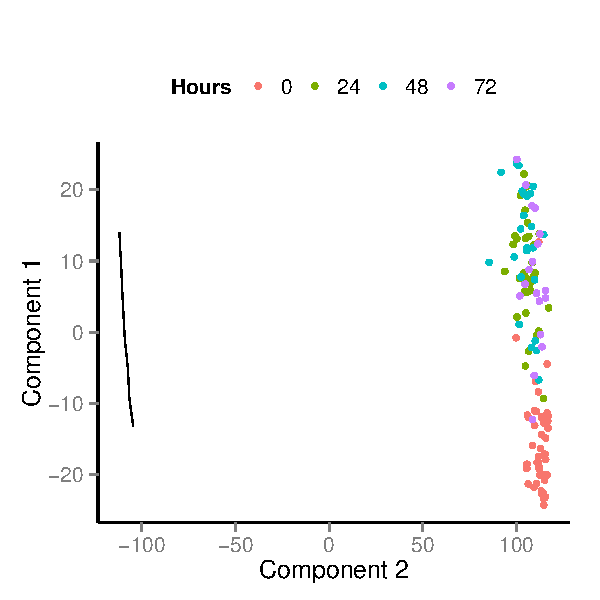
\includegraphics[width=\maxwidth]{figure/plot_ordering_mst-1} 

}



\end{knitrout}

To confirm that the ordering is correct, and to verify that we don't need to flip around the ordering using the \Robject{reverse} flag in \Robject{orderCells}, we can select a couple of markers of myogenic progress. Plotting these genes demonstrates that ordering looks good: 
\begin{knitrout}
\definecolor{shadecolor}{rgb}{0.969, 0.969, 0.969}\color{fgcolor}\begin{kframe}
\begin{alltt}
\hlstd{HSMM_filtered} \hlkwb{<-} \hlstd{HSMM_myo[expressed_genes,]}

\hlstd{my_genes} \hlkwb{<-} \hlkwd{row.names}\hlstd{(}\hlkwd{subset}\hlstd{(}\hlkwd{fData}\hlstd{(HSMM_filtered),}
                             \hlstd{gene_short_name} \hlopt \hlkwd{c}\hlstd{(}\hlstr{"CDK1"}\hlstd{,} \hlstr{"MEF2C"}\hlstd{,} \hlstr{"MYH3"}\hlstd{)))}

\hlstd{cds_subset} \hlkwb{<-} \hlstd{HSMM_filtered[my_genes,]}
\hlkwd{plot_genes_in_pseudotime}\hlstd{(cds_subset,} \hlkwc{color_by}\hlstd{=}\hlstr{"Hours"}\hlstd{)}
\end{alltt}
\end{kframe}

{\centering 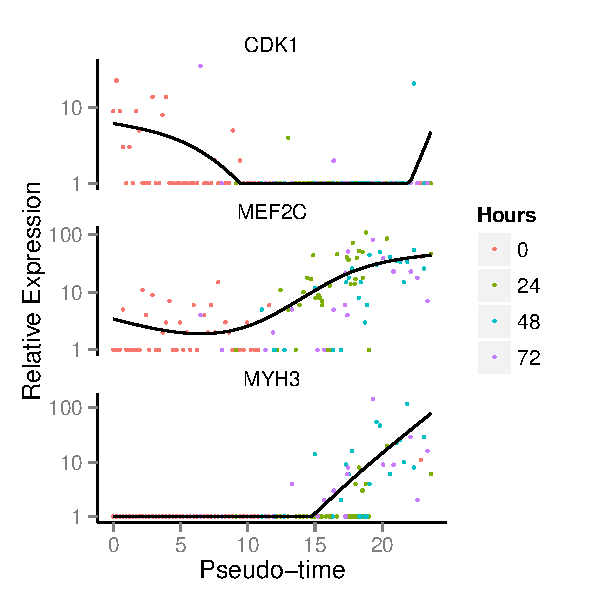
\includegraphics[width=\maxwidth]{figure/plot_markers-1} 

}



\end{knitrout}

\section{Advanced differential expression analysis}

In this section, we'll explore how to use Monocle to find genes that are differentially expressed according to several different criteria. First, we'll look at how to use our previous classification of the cells by type to find genes that distinguish fibroblasts and myoblasts. Second, we'll look at how to find genes that are differentially expressed as a function of pseudotime, such as those that become activated or repressed during differentiation.  Finally, you'll see how to perform multi-factorial differential analysis, which can help subtract the effects of confounding variables in your experiment.  

To keep the vignette simple and fast, we'll be working with small sets of genes. Rest assured, however, that Monocle can analyze many thousands of genes even in large experiments, making it useful for discovering dynamically regulated genes during the biological process you're studying.

\subsection{Finding genes that distinguish cell type or state}

During a dynamic biological process such as differentiation, cells might assume distinct intermediate or final states.  Recall that earlier we distinguished myoblasts from contaminating fibroblasts on the basis of several key markers. Let's look at several other genes that should distinguish between fibroblasts and myoblasts. 
\begin{knitrout}
\definecolor{shadecolor}{rgb}{0.969, 0.969, 0.969}\color{fgcolor}\begin{kframe}
\begin{alltt}
\hlstd{to_be_tested} \hlkwb{<-} \hlkwd{row.names}\hlstd{(}\hlkwd{subset}\hlstd{(}\hlkwd{fData}\hlstd{(HSMM),}
                             \hlstd{gene_short_name} \hlopt \hlkwd{c}\hlstd{(}\hlstr{"UBC"}\hlstd{,} \hlstr{"NCAM1"}\hlstd{,} \hlstr{"ANPEP"}\hlstd{)))}
\hlstd{cds_subset} \hlkwb{<-} \hlstd{HSMM[to_be_tested,]}
\end{alltt}
\end{kframe}
\end{knitrout}

To test the effects of \Robject{CellType} on gene expression, we simply call \Rfunction{differentialGeneTest} on the genes we've selected. However, we have to specify a \emph{model formula} in the call to tell Monocle that we care about genes with expression levels that depends on \emph{CellType}.  Monocle's differential expression analysis works essentially by fitting two models to the expression values for each gene, working through each gene independently.  The first of the two models is called the \emph{full} model.  This model is essentially a way of predicting the expression value of each gene in a given cell knowing only whether that cell is a fibroblast or a myoblast.  The second model, called the \emph{reduced} model, does the same thing, but it doesn't know the \Robject{CellType} for each cell.  It has to come up with a reasonable prediction of the expression value for the gene that will be used for \emph{all} the cells. Because the full model has more information about each cell, it will do a better job of predicting the expression of the gene in each cell.  The question Monocle must answer for each gene is \emph{how much better} the full model's prediction is than the reduced model's. The greater the improvement that comes from knowing the \Robject{CellType} of each cell, the more significant the differential expression result. This is a common strategy in differential analysis, and we leave a detailed statistical exposition of such methods to others.

To set up the test based on \Robject{CellType}, we simply call \Rfunction{differentialGeneTest} with a string specifying \Robject{fullModelFormulaStr}.  We don't have to specify the reduced model in this case, because the default of \Robject{~1} is what we want here.

\begin{knitrout}
\definecolor{shadecolor}{rgb}{0.969, 0.969, 0.969}\color{fgcolor}\begin{kframe}
\begin{alltt}
\hlstd{diff_test_res} \hlkwb{<-} \hlkwd{differentialGeneTest}\hlstd{(cds_subset,} \hlkwc{fullModelFormulaStr}\hlstd{=}\hlstr{"~CellType"}\hlstd{, )}
\hlstd{diff_test_res[,}\hlkwd{c}\hlstd{(}\hlstr{"gene_short_name"}\hlstd{,} \hlstr{"pval"}\hlstd{,} \hlstr{"qval"}\hlstd{)]}
\end{alltt}
\begin{verbatim}
##                    gene_short_name         pval         qval
## ENSG00000149294.12           NCAM1 1.082374e-24 3.247121e-24
## ENSG00000150991.10             UBC 1.547155e-01 1.547155e-01
## ENSG00000166825.9            ANPEP 8.423212e-06 1.263482e-05
\end{verbatim}
\end{kframe}
\end{knitrout}

Note that all the genes are significantly differentially expressed as a function of \Robject{CellType} except the housekeeping gene TBP, which we're using a negative control.  However, we don't know which genes correspond to myoblast-specific genes (those more highly expressed in myoblasts versus fibroblast specific genes.  We can again plot them with a jitter plot to see:

\begin{knitrout}
\definecolor{shadecolor}{rgb}{0.969, 0.969, 0.969}\color{fgcolor}\begin{kframe}
\begin{alltt}
\hlkwd{plot_genes_jitter}\hlstd{(cds_subset,} \hlkwc{grouping}\hlstd{=}\hlstr{"CellType"}\hlstd{,} \hlkwc{color_by}\hlstd{=}\hlstr{"CellType"}\hlstd{,}
                  \hlkwc{nrow}\hlstd{=}\hlnum{1}\hlstd{,} \hlkwc{ncol}\hlstd{=}\hlkwa{NULL}\hlstd{,} \hlkwc{plot_trend}\hlstd{=}\hlnum{TRUE}\hlstd{)}
\end{alltt}


{\ttfamily\noindent\itshape\color{messagecolor}{\#\# geom\_path: Each group consist of only one observation. Do you need to adjust the group aesthetic?\\\#\# geom\_path: Each group consist of only one observation. Do you need to adjust the group aesthetic?\\\#\# geom\_path: Each group consist of only one observation. Do you need to adjust the group aesthetic?}}\end{kframe}

{\centering 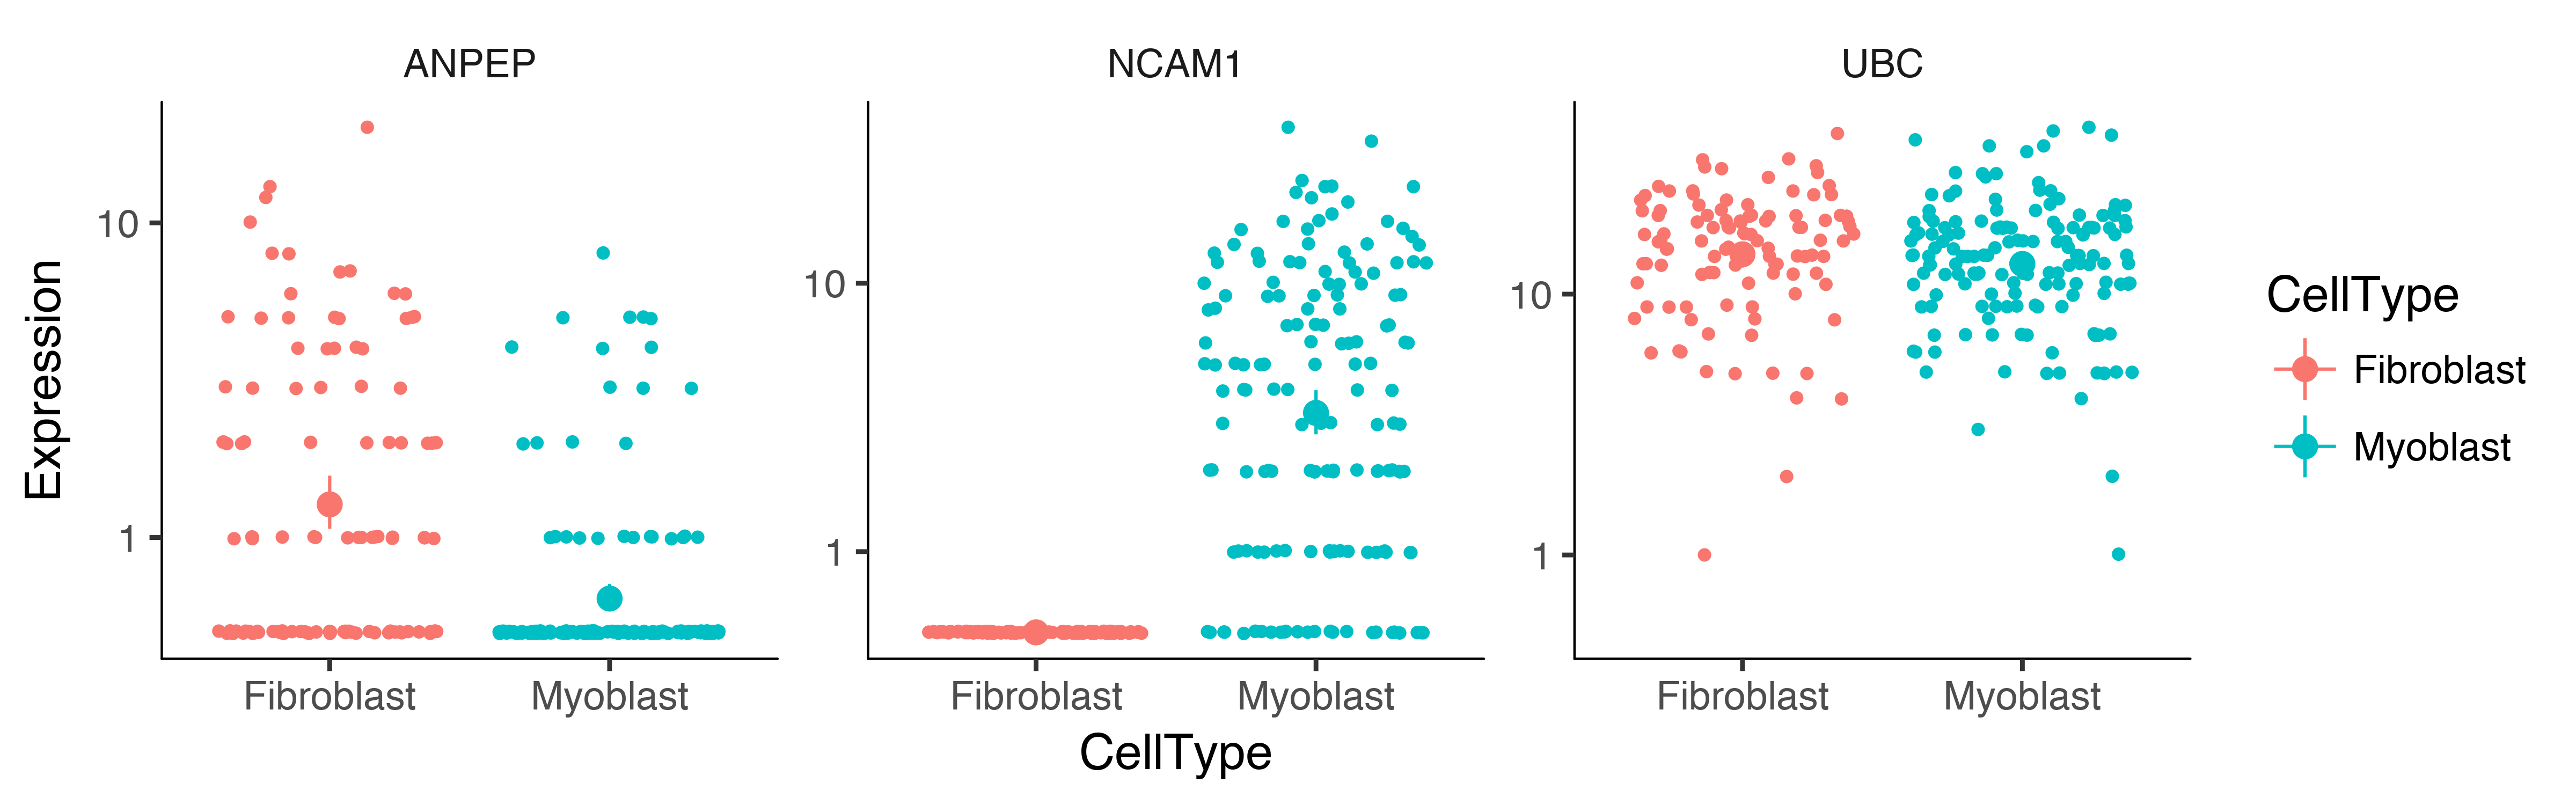
\includegraphics[width=\maxwidth]{figure/jitter_plot_diff_res-1} 

}



\end{knitrout}

Note that we could also simply compute summary statistics such as mean or median expression level on a per-\Robject{CellType} basis to see this, which might be handy if we are looking at more than a handful of genes. Of course, we could test for genes that change as a function of \Robject{Hours} to find time-varying genes, or \Robject{Media} to identify genes that are responsive to the serum switch.  In general, model formulae can contain terms in the pData table of the CellDataSet. 

The \Rfunction{differentialGeneTest} function is actually quite simple ``under the hood''.  The call above is equivalent to:
\begin{knitrout}
\definecolor{shadecolor}{rgb}{0.969, 0.969, 0.969}\color{fgcolor}\begin{kframe}
\begin{alltt}
\hlstd{full_model_fits} \hlkwb{<-} \hlkwd{fitModel}\hlstd{(cds_subset,}  \hlkwc{modelFormulaStr}\hlstd{=}\hlstr{"~CellType"}\hlstd{)}
\hlstd{reduced_model_fits} \hlkwb{<-} \hlkwd{fitModel}\hlstd{(cds_subset,} \hlkwc{modelFormulaStr}\hlstd{=}\hlstr{"~1"}\hlstd{)}
\hlstd{diff_test_res} \hlkwb{<-} \hlkwd{compareModels}\hlstd{(full_model_fits, reduced_model_fits)}
\hlstd{diff_test_res}
\end{alltt}
\end{kframe}
\end{knitrout}
Occassionally, as we'll see later, it's useful to be able to call \Rfunction{fitModel} directly.

\subsection{Finding genes that change as a function of pseudotime}

Monocle's main job is to put cells in order of progress through a biological process (such as cell differentiation) without knowing which genes to look at ahead of time.  Once it's done so, you can analyze the cells to find genes that changes as the cells make progress.  For example, you can find genes that are significantly upregulated as the cells ``mature''.  Let's look at a panel of genes important for myogenesis: 

\begin{knitrout}
\definecolor{shadecolor}{rgb}{0.969, 0.969, 0.969}\color{fgcolor}\begin{kframe}
\begin{alltt}
\hlstd{to_be_tested} \hlkwb{<-} \hlkwd{row.names}\hlstd{(}\hlkwd{subset}\hlstd{(}\hlkwd{fData}\hlstd{(HSMM),}
                             \hlstd{gene_short_name} \hlopt \hlkwd{c}\hlstd{(}\hlstr{"MYH3"}\hlstd{,} \hlstr{"MEF2C"}\hlstd{,} \hlstr{"CCNB2"}\hlstd{,} \hlstr{"TNNT1"}\hlstd{)))}
\hlstd{cds_subset} \hlkwb{<-} \hlstd{HSMM_myo[to_be_tested,]}
\end{alltt}
\end{kframe}
\end{knitrout}

Again, we'll need to specify the model we want to use for differential analysis.  This model will be a bit more complicated than the one we used to look at the differences between \Robject{CellType}.  Monocle assigns each cell a ``pseudotime'' value, which records its progress through the process in the experiment.  The model can test against changes as a function of this value. Monocle uses the \Rpackage{VGAM} package to model a gene's expression level as a smooth, nonlinear function of pseudotime:
\begin{knitrout}
\definecolor{shadecolor}{rgb}{0.969, 0.969, 0.969}\color{fgcolor}\begin{kframe}
\begin{alltt}
\hlstd{diff_test_res} \hlkwb{<-} \hlkwd{differentialGeneTest}\hlstd{(cds_subset,}  \hlkwc{fullModelFormulaStr}\hlstd{=}\hlstr{"~sm.ns(Pseudotime)"}\hlstd{)}
\end{alltt}
\end{kframe}
\end{knitrout}

The \Rfunction{sm.ns} function states that Monocle should fit a natural spline through the expression values to help it describe the changes in expression as a function of progress. We'll see what this trend looks like in just a moment. Other smoothing functions are available.

Once again, let's add in the gene annotations so it's easy to see which genes are significant.
\begin{knitrout}
\definecolor{shadecolor}{rgb}{0.969, 0.969, 0.969}\color{fgcolor}\begin{kframe}
\begin{alltt}
\hlstd{diff_test_res[,}\hlkwd{c}\hlstd{(}\hlstr{"gene_short_name"}\hlstd{,} \hlstr{"pval"}\hlstd{,} \hlstr{"qval"}\hlstd{)]}
\end{alltt}
\begin{verbatim}
##                    gene_short_name         pval         qval
## ENSG00000081189.9            MEF2C 1.446638e-20 5.786550e-20
## ENSG00000105048.12           TNNT1 1.991870e-10 2.655826e-10
## ENSG00000109063.9             MYH3 7.207879e-19 1.441576e-18
## ENSG00000157456.3            CCNB2 3.777935e-06 3.777935e-06
\end{verbatim}
\end{kframe}
\end{knitrout}

We can plot the expression levels of these genes, all of which show significant changes as a function of differentiation, using the function \Rfunction{plot\_genes\_in\_pseudotime}. This function has a number of cosmetic options you can use to control the layout and appearance of your plot.

\begin{knitrout}
\definecolor{shadecolor}{rgb}{0.969, 0.969, 0.969}\color{fgcolor}\begin{kframe}
\begin{alltt}
\hlkwd{plot_genes_in_pseudotime}\hlstd{(cds_subset,} \hlkwc{color_by}\hlstd{=}\hlstr{"Hours"}\hlstd{)}
\end{alltt}
\end{kframe}

{\centering 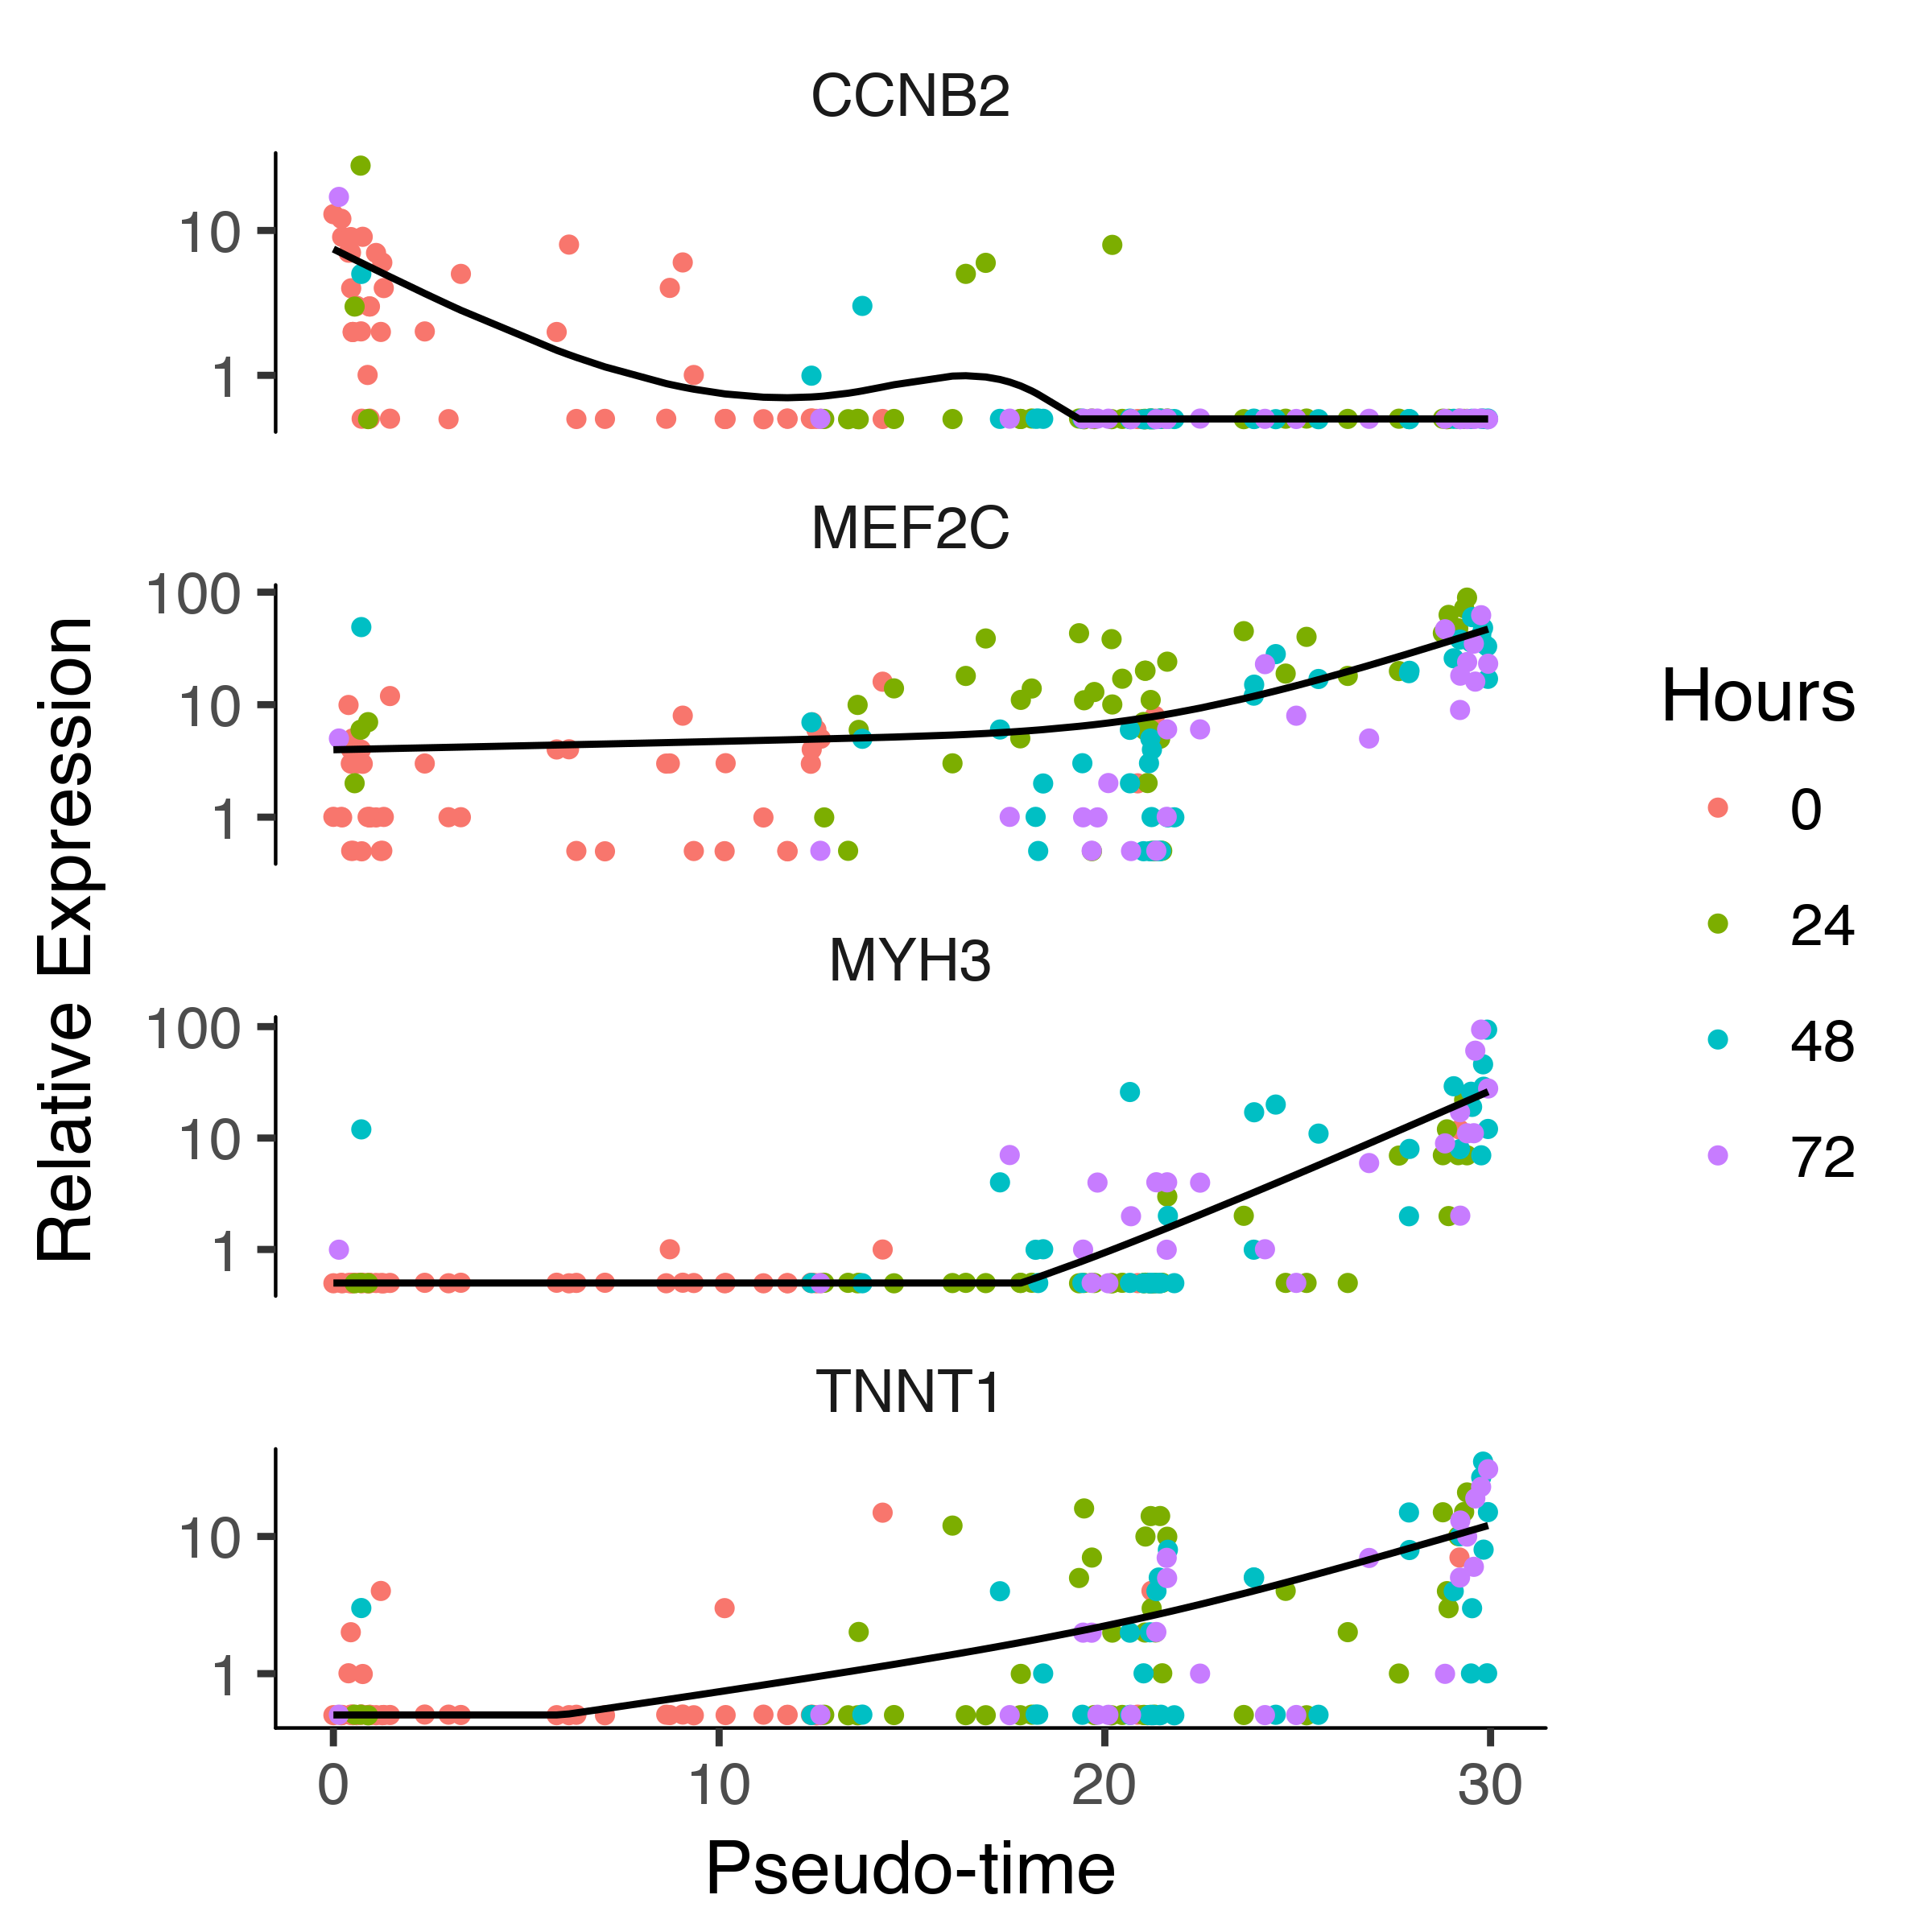
\includegraphics[width=\maxwidth]{figure/plot_diff_res_pt-1} 

}



\end{knitrout}

\subsection{Multi-factorial differential expression analysis}

Monocle can perform differential analysis in the presence of multiple factors, which can help you subtract some factors to see the effects of others.  In the simple example below, Monocle tests three genes for differential expression between myoblasts and fibroblasts, while subtracting the effect of \Robject{Hours}, which encodes the day on which each cell was collected. To do this, we must specify both the full model and the reduced model. The full model captures the effects of both \Robject{CellType} and \Robject{Hours}, while the reduced model only knows about \Robject{Hours}.  

When we plot the expression levels of these genes, we can modify the resulting object returned by \Rfunction{plot\_genes\_jitter} to allow them to have independent y-axis ranges, to better highlight the differences between cell states.

\begin{knitrout}
\definecolor{shadecolor}{rgb}{0.969, 0.969, 0.969}\color{fgcolor}\begin{kframe}
\begin{alltt}
\hlstd{to_be_tested} \hlkwb{<-} \hlkwd{row.names}\hlstd{(}\hlkwd{subset}\hlstd{(}\hlkwd{fData}\hlstd{(HSMM),}
                             \hlstd{gene_short_name} \hlopt \hlkwd{c}\hlstd{(}\hlstr{"TPM1"}\hlstd{,} \hlstr{"MYH3"}\hlstd{,} \hlstr{"CCNB2"}\hlstd{,} \hlstr{"GAPDH"}\hlstd{)))}
\hlstd{cds_subset} \hlkwb{<-} \hlstd{HSMM[to_be_tested,]}

\hlstd{diff_test_res} \hlkwb{<-} \hlkwd{differentialGeneTest}\hlstd{(cds_subset,}
                                      \hlkwc{fullModelFormulaStr}\hlstd{=}\hlstr{"~CellType + Hours"}\hlstd{,}
                                      \hlkwc{reducedModelFormulaStr}\hlstd{=}\hlstr{"~Hours"}\hlstd{)}
\hlstd{diff_test_res[,}\hlkwd{c}\hlstd{(}\hlstr{"gene_short_name"}\hlstd{,} \hlstr{"pval"}\hlstd{,} \hlstr{"qval"}\hlstd{)]}
\end{alltt}
\begin{verbatim}
##                    gene_short_name         pval         qval
## ENSG00000109063.9             MYH3 2.788118e-15 1.115247e-14
## ENSG00000111640.10           GAPDH 6.293919e-01 6.293919e-01
## ENSG00000140416.15            TPM1 1.788738e-12 3.577477e-12
## ENSG00000157456.3            CCNB2 3.968834e-02 5.291779e-02
\end{verbatim}
\begin{alltt}
\hlkwd{plot_genes_jitter}\hlstd{(cds_subset,}
                  \hlkwc{grouping}\hlstd{=}\hlstr{"Hours"}\hlstd{,} \hlkwc{color_by}\hlstd{=}\hlstr{"CellType"}\hlstd{,} \hlkwc{plot_trend}\hlstd{=}\hlnum{TRUE}\hlstd{)} \hlopt{+}
  \hlkwd{facet_wrap}\hlstd{(} \hlopt{~} \hlstd{feature_label,} \hlkwc{scales}\hlstd{=}\hlstr{"free_y"}\hlstd{)}
\end{alltt}
\end{kframe}

{\centering 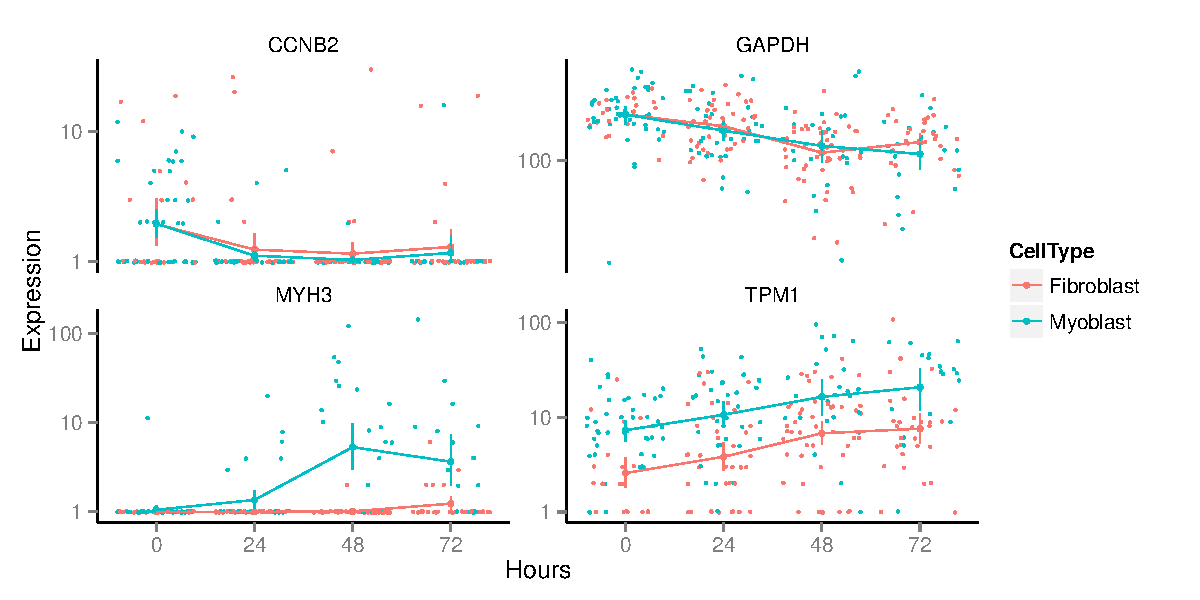
\includegraphics[width=\maxwidth]{figure/plot_diff_res_multi-1} 

}



\end{knitrout}

\section{Clustering genes by pseudotemporal expression pattern}

A common question that arises when studying time-series gene expression studies is: ``which genes follow similar kinetic trends''?  Monocle can help you answer this question by grouping genes that have similar trends, so you can analyze these groups to see what they have in common.  To do this, we'll first fit a smooth curve for each gene's expression trend as a function of pseudotime, then we'll group the genes according to similarity of these curves. 

We start by using the model fitting function that's used during differential expression testing.  This fitting procedure works gene by gene and can take a while, so we'll just work with 100 randomly chosen genes to keep the vignette small and fast.

\begin{knitrout}
\definecolor{shadecolor}{rgb}{0.969, 0.969, 0.969}\color{fgcolor}\begin{kframe}
\begin{alltt}
\hlstd{sampled_gene_cds} \hlkwb{<-} \hlstd{HSMM_filtered[}\hlkwd{sample}\hlstd{(}\hlkwd{nrow}\hlstd{(}\hlkwd{fData}\hlstd{(HSMM_filtered)),} \hlnum{100}\hlstd{),]}
\hlstd{full_model_fits} \hlkwb{<-} \hlkwd{fitModel}\hlstd{(sampled_gene_cds,}  \hlkwc{modelFormulaStr}\hlstd{=}\hlstr{"~sm.ns(Pseudotime, df=3)"}\hlstd{)}
\end{alltt}
\end{kframe}
\end{knitrout}

The \Robject{full\_model\_fits} list contains a model for each gene that we've chosen.  We can generate a matrix of values where each row holds the predicted exression values for a gene over each cell, which correspond to the columns. Monocle provides the \Rfunction{responseMatrix} function to make this easy.

\begin{knitrout}
\definecolor{shadecolor}{rgb}{0.969, 0.969, 0.969}\color{fgcolor}\begin{kframe}
\begin{alltt}
\hlstd{expression_curve_matrix} \hlkwb{<-} \hlkwd{responseMatrix}\hlstd{(full_model_fits)}
\hlkwd{dim}\hlstd{(expression_curve_matrix)}
\end{alltt}
\begin{verbatim}
## [1] 100 120
\end{verbatim}
\end{kframe}
\end{knitrout}

Now we'll feed this matrix to a function, \Rfunction{clusterGenes}, that will cluster the genes into four groups:

\begin{knitrout}
\definecolor{shadecolor}{rgb}{0.969, 0.969, 0.969}\color{fgcolor}\begin{kframe}
\begin{alltt}
\hlstd{clusters} \hlkwb{<-} \hlkwd{clusterGenes}\hlstd{(expression_curve_matrix,} \hlkwc{k}\hlstd{=}\hlnum{4}\hlstd{)}
\hlkwd{plot_clusters}\hlstd{(HSMM_filtered, clusters)}
\end{alltt}


{\ttfamily\noindent\color{warningcolor}{\#\# Warning: 'str\_join' is deprecated.\\\#\# Use 'str\_c' instead.\\\#\# See help("{}Deprecated"{})}}\end{kframe}

{\centering 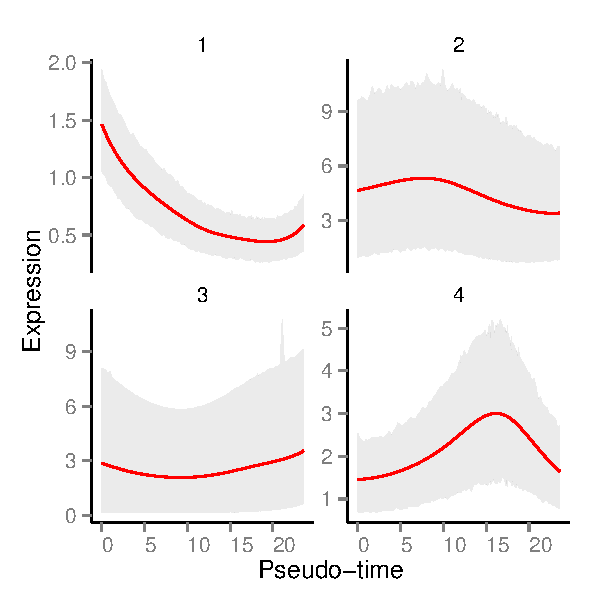
\includegraphics[width=\maxwidth]{figure/cluster_and_plot-1} 

}



\end{knitrout}

The \Rfunction{plot\_clusters} function returns a ggplot2 object showing the shapes of the expression patterns followed by the 100 genes we've picked out.  The topographic lines highlight the distributions of the kinetic patterns relative to the overall trend lines, shown in red.

%\section{Using Monocle with qPCR data}

\section{Citation}
If you use Monocle to analyze your experiments, please cite:
\begin{knitrout}
\definecolor{shadecolor}{rgb}{0.969, 0.969, 0.969}\color{fgcolor}\begin{kframe}
\begin{alltt}
\hlkwd{citation}\hlstd{(}\hlstr{"monocle"}\hlstd{)}
\end{alltt}
\begin{verbatim}
## 
##   Cole Trapnell and Davide Cacchiarelli et al (2014): The dynamics
##   and regulators of cell fate decisions are revealed by
##   pseudo-temporal ordering of single cells. Nature Biotechnology
## 
## A BibTeX entry for LaTeX users is
## 
##   @Article{,
##     title = {The dynamics and regulators of cell fate decisions are revealed by pseudo-temporal ordering of single cells},
##     author = {Cole Trapnell and Davide Cacchiarelli and Jonna Grimsby and Prapti Pokharel and Shuqiang Li and Michael Morse and Niall J. Lennon and Kenneth J. Livak and Tarjei S. Mikkelsen and John L. Rinn},
##     year = {2014},
##     journal = {Nature Biotechnology},
##   }
\end{verbatim}
\end{kframe}
\end{knitrout}

\section{Acknowledgements}

Monocle was built by Cole Trapnell and Davide Cacchiarelli, with substantial design input John Rinn and Tarjei Mikkelsen. We are grateful to Sharif Bordbar, Chris Zhu, Amy Wagers and the Broad RNAi platform for technical assistance, and Magali Soumillon for helpful discussions. Cole Trapnell is a Damon Runyon Postdoctoral Fellow. Davide Cacchiarelli is a Human Frontier Science Program Fellow. Cacchiarelli and Mikkelsen were supported by the Harvard Stem Cell Institute. John Rinn is the Alvin and Esta Star Associate Professor. This work was supported by NIH grants 1DP2OD00667, P01GM099117, and P50HG006193-01. This work was also supported in part by the Single Cell Genomics initiative, a collaboration between the Broad Institute and Fluidigm Inc. This vignette was created from Wolfgang Huber's Bioconductor vignette style document, and patterned after the vignette for \Rpackage{DESeq}, by Simon Anders and Wolfgang Huber.

\section{Session Info}
\begin{knitrout}
\definecolor{shadecolor}{rgb}{0.969, 0.969, 0.969}\color{fgcolor}\begin{kframe}
\begin{alltt}
\hlkwd{sessionInfo}\hlstd{()}
\end{alltt}
\begin{verbatim}
## R version 3.2.1 (2015-06-18)
## Platform: x86_64-apple-darwin13.4.0 (64-bit)
## Running under: OS X 10.10.5 (Yosemite)
## 
## locale:
## [1] en_US.UTF-8/en_US.UTF-8/en_US.UTF-8/C/en_US.UTF-8/en_US.UTF-8
## 
## attached base packages:
##  [1] grid      splines   stats4    parallel  stats     graphics  grDevices
##  [8] utils     datasets  methods   base     
## 
## other attached packages:
##  [1] Hmisc_3.17-0           Formula_1.2-1          survival_2.38-3       
##  [4] lattice_0.20-33        monocle_1.99.0         VGAM_1.0-0            
##  [7] HSMMSingleCell_0.102.0 ggplot2_1.0.1          reshape2_1.4.1        
## [10] Biobase_2.28.0         BiocGenerics_0.14.0    knitr_1.11            
## 
## loaded via a namespace (and not attached):
##  [1] Rcpp_0.12.1         formatR_1.2         RColorBrewer_1.1-2 
##  [4] plyr_1.8.3          highr_0.5           tools_3.2.1        
##  [7] rpart_4.1-10        digest_0.6.8        evaluate_0.7.2     
## [10] gtable_0.1.2        Matrix_1.2-2        igraph_1.0.1       
## [13] DBI_0.3.1           proto_0.3-10        gridExtra_2.0.0    
## [16] fastICA_1.2-0       stringr_1.0.0       dplyr_0.4.3        
## [19] cluster_2.0.3       nnet_7.3-11         combinat_0.0-8     
## [22] R6_2.1.1            foreign_0.8-66      pheatmap_1.0.7     
## [25] latticeExtra_0.6-26 limma_3.24.15       irlba_2.0.0        
## [28] magrittr_1.5        scales_0.3.0        matrixStats_0.15.0 
## [31] MASS_7.3-44         assertthat_0.1      colorspace_1.2-6   
## [34] labeling_0.3        stringi_1.0-1       acepack_1.3-3.3    
## [37] munsell_0.4.2
\end{verbatim}
\end{kframe}
\end{knitrout}

\bibliographystyle{unsrt}
\bibliography{monocle_alg}

\end{document}
